\section{Applications}

Figure \ref{boat-sample} shows a basic usage case of our method.
A boat is floating on the sea; a pack of heavy balls are spawning above the boat and falling into it.
Without having to write any additional codes, just by keeping loading heavy balls onto the boat, the sunk depth of the boat automatically increases.

\begin{figure}[H]
	\centering
	\begin{subcaptionblock}{0.46\textwidth}
		\centering
		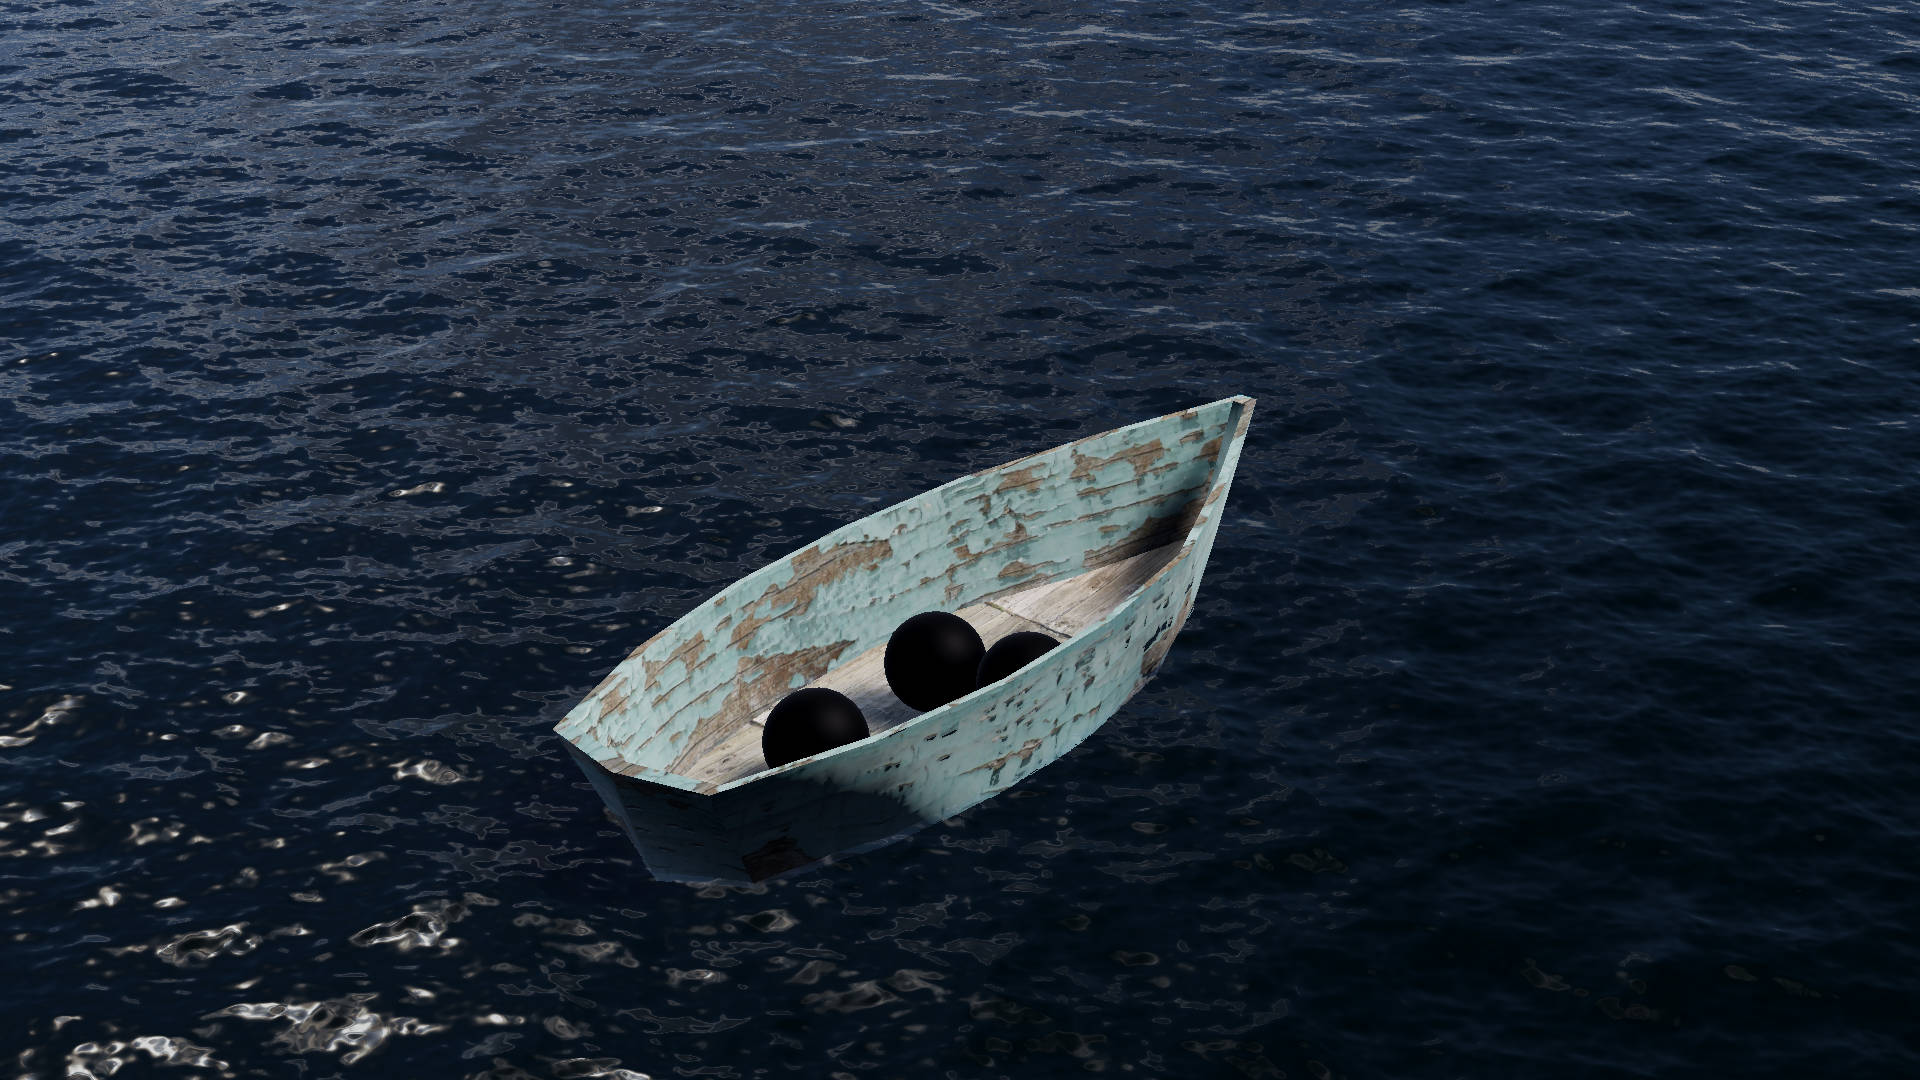
\includegraphics[width=0.9\textwidth]{../Thesis/figures/light-boat.jpg}
		\caption{A boat containing a few balls.}
	\end{subcaptionblock}
	\begin{subcaptionblock}{0.46\textwidth}
		\centering
		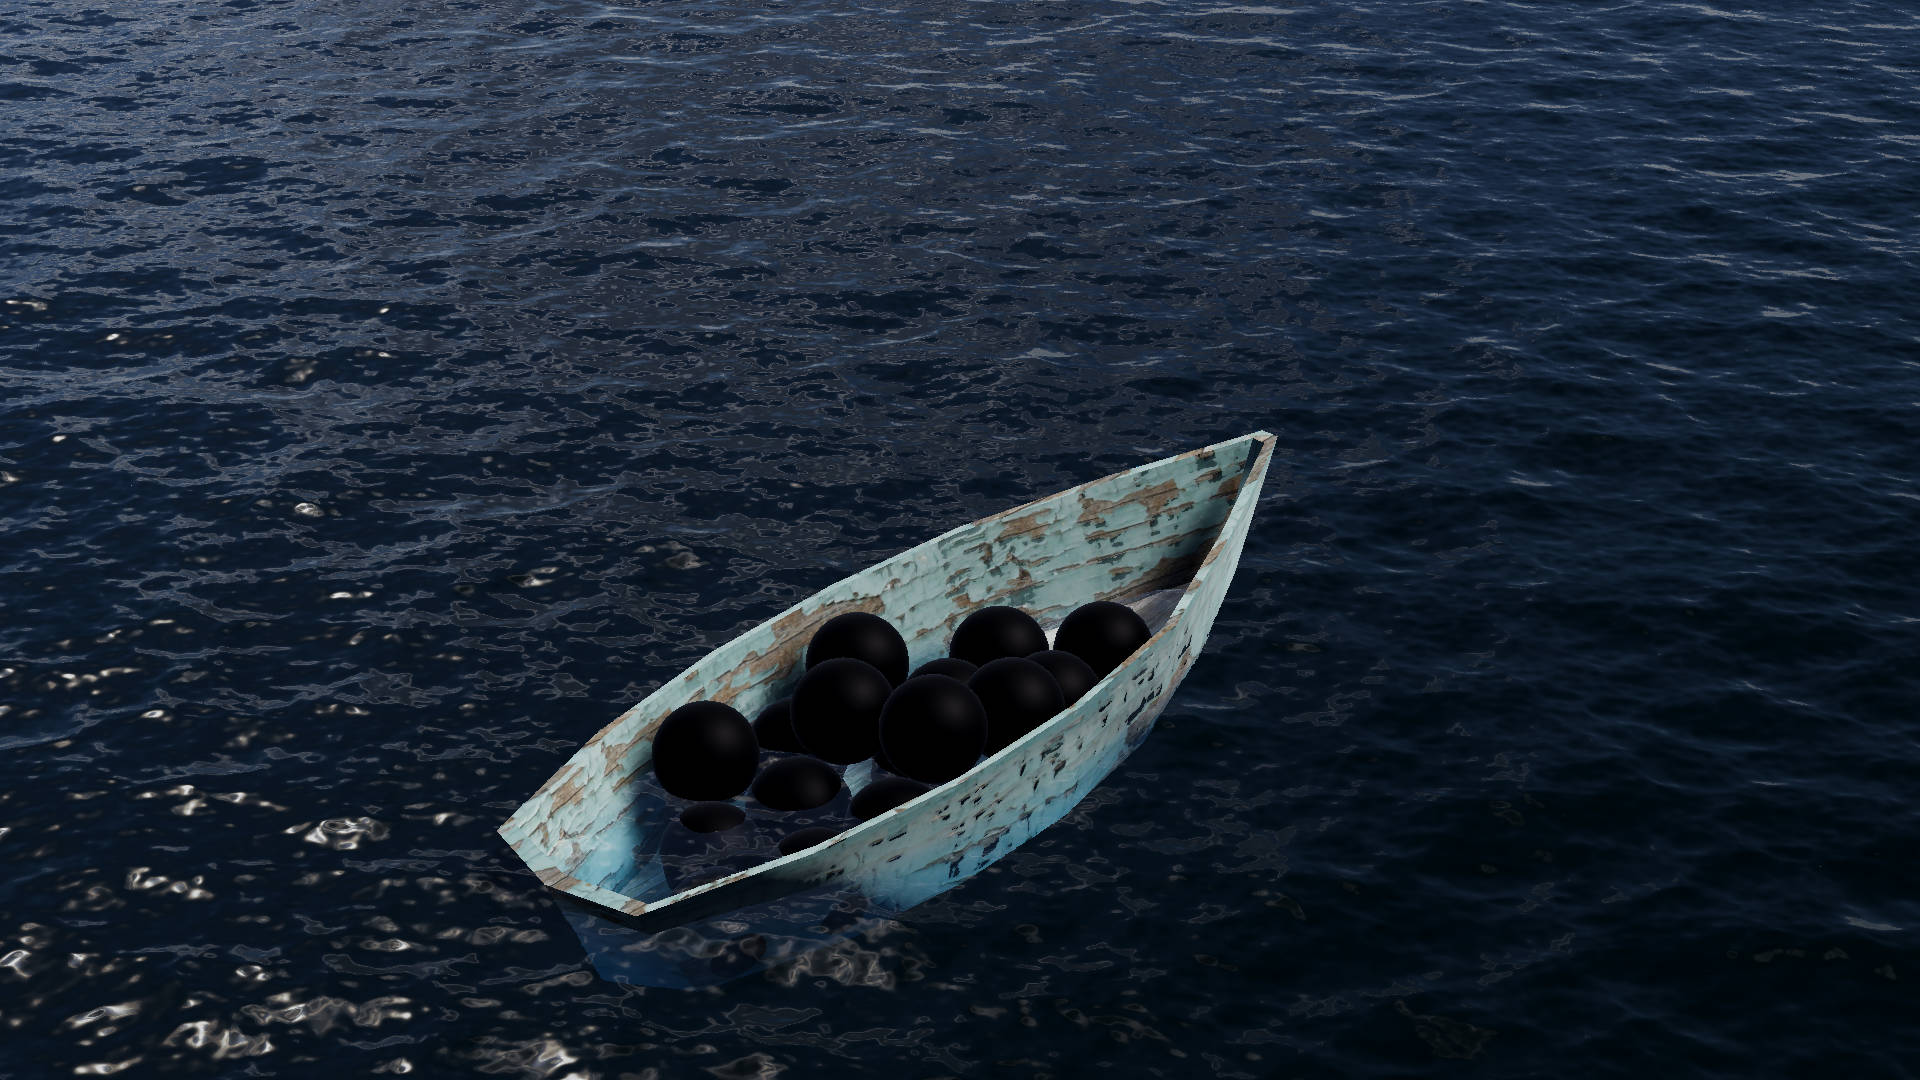
\includegraphics[width=0.9\textwidth]{../Thesis/figures/heavy-boat.jpg}
		\caption{The same boat containing many balls.}
	\end{subcaptionblock}
	\caption{Loading more balls onto the boat increases its depth.}
	\label{boat-sample}
\end{figure}

When applied in real game design, this extra freedom could allow game designers to create more complex mechanisms.
It is clear that often an open mechanism tends to lead to emergent behaviors \cite{sweetser2006emergent}, thus increasing the fun of the game.

Buoyancy simulation could also be used for creating the vibes.
Figure \ref{floating-donut-in-game} shows a screenshot of a poolcore-themed puzzle game, in which water is a main part of the visual design.
Adding objects that could float on water definitely helps emphasize the vibes of the pools.

\begin{figure}[H]
	\centering
	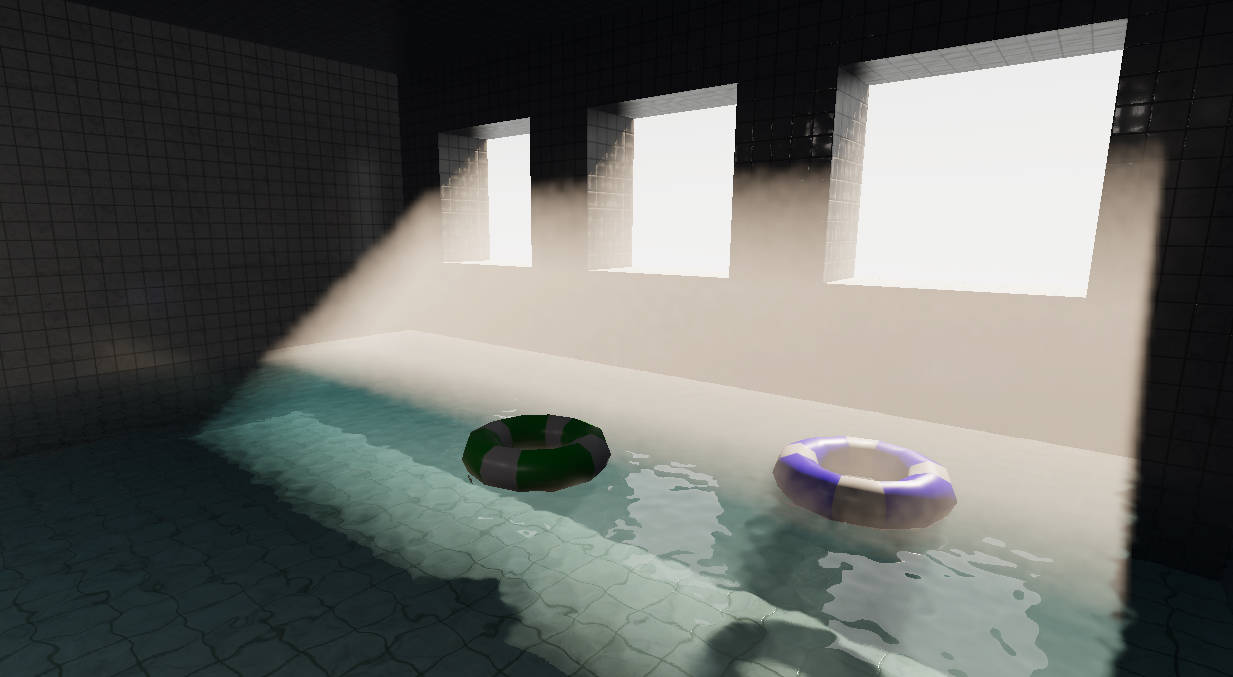
\includegraphics[width=0.4\textwidth]{../Thesis/figures/floating-donut-in-game.jpg}
	\caption{Floating objects can be seen in a poolcore-themed game.}
	\label{floating-donut-in-game}
\end{figure}